%%%%%%%%%%%%%%%%%%%%%%%%%%%%%%%%%%%%%%%%%%%%%%%%%%%%%%%%%%%%%%%%%%%%
\section{Data Acquisition System (DAQ) Overview (Georgia Karagiorgi)}
\label{sec:fdsp-daq-ov}

\metainfo{2 Pages - largely generic but some highlighting of SP-specifics.}

%%%%%%%%%%%%%%%%%%%%%%%%%%%%%%%%%
\subsection{Introduction}
\label{sec:fdsp-daq-intro}

The overall DUNE Far Detector Data Acquisition System (DAQ) is
illustrated in Fig.~\ref{fig:daq-overview}.
\fixme{Describe figure here.}

Figure.~\ref{fig:daq-overview} illustrates the data flow and the
exchange of trigger and monitoring messages.



\begin{dunefigure}[DAQ Overview]{fig:daq-overview}
  {An overview of high-level DAQ components and their connections for the full Far Detector with details showing the multiplicity of front ends for the Single-Phase \SI{10}{\kton} module.}
% This PDF is made from the .dot of the same name.
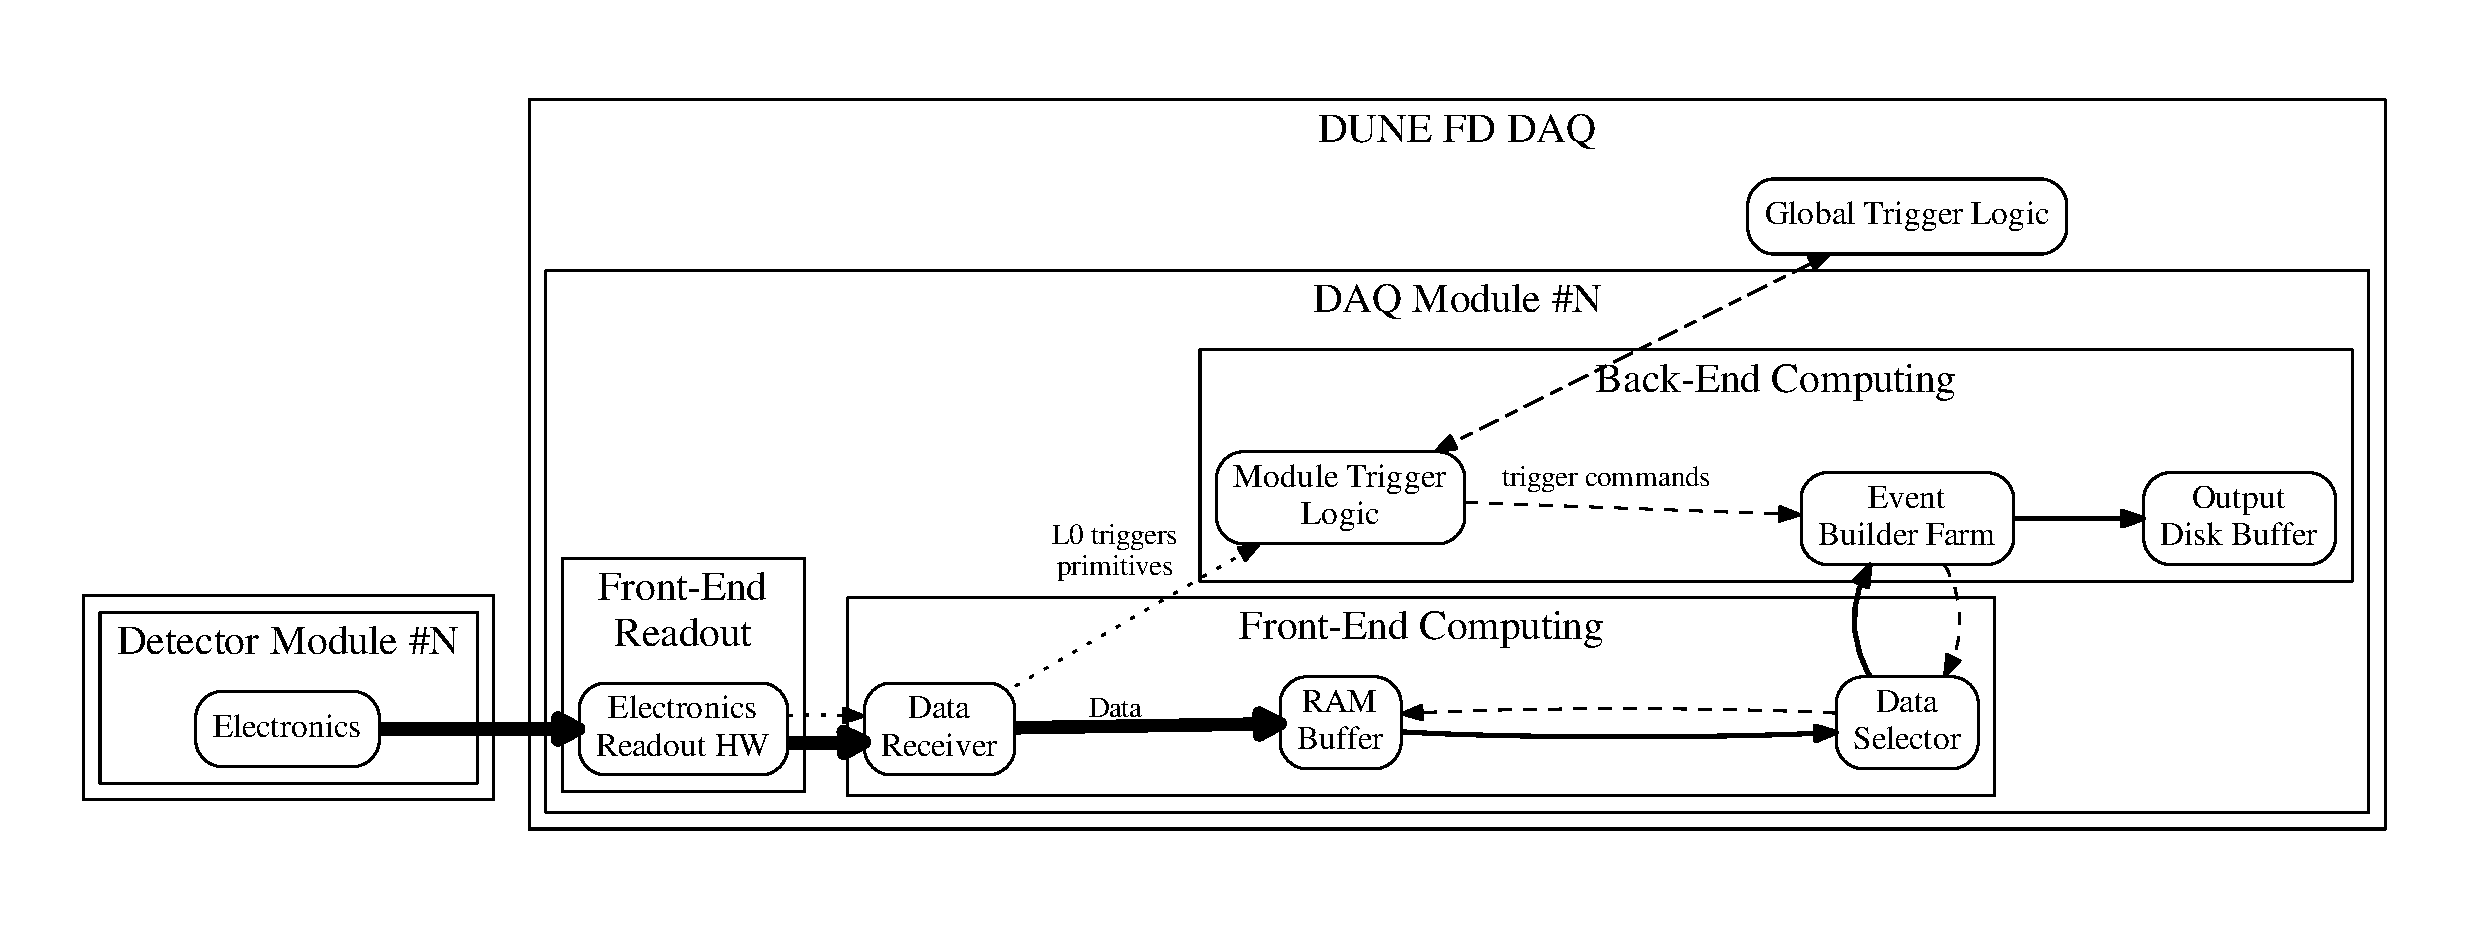
\includegraphics[width=0.8\textwidth]{daq-overview.pdf}%
\end{dunefigure}


%%%%%%%%%%%%%%%%%%%%%%%%%%%%%%%%%%%%%

\subsection{Design Considerations}
\label{sec:fdsp-daq-des-consid}


\metainfo{Include: Raw data rate from WIBs, Josh's table of data volumes for each event type and the 30 PB/year offline limit. Space and thermal power limits.  Note, this table may be better put into Section~\ref{sec:fdsp-daq-design} to make this section more generic.}


The Data Acquisition System design must enable... 
...

\fixme{Anne suggests: Within this section add ref to requirements document when it's ready, and maybe list the most important half dozen in a table here). E.g.,}  

\begin{dunetable}
[Important requirements on the DAQ system design]
{p{0.8\textwidth}}
{pdphysicsparams}
{Important requirements on the DAQ system design}   
Requirement  \\ \toprowrule
  \\ \colhline
   \\ \colhline
 ...\\ 
\end{dunetable}

\fixme{By the end of the volume, for every requirement listed in this section, there should exist an explanation of how it will be satisfied.}


%%%%%%%%%%%%%%%%%%%%%%%%%%%%%%%%
\subsection{Scope}
\label{sec:fdsp-daq-scope}

\metainfo{This section may also wish to refer to Fig.~\ref{fig:daq-overview}.}

The scope of the Data Acquisition System includes the continued procurement of materials for, and the fabrication, testing, delivery and installation of the following systems: 

\fixme{Whatever the items are...}

\begin{itemize}
\item Readout electronics 
\item 
\end{itemize}


\newpage 
